\chapter{Montagem do Robô} \label{ch:mount-robot}
\section{Modelagem da Base do Robô}
Foi adquirida uma placa de aço de dimensões 500 mm de largura 900 mm de comprimento e 1,6 mm de espessura. Para se adequar ao projeto a placa foi reduzida para a seguinte dimensão 520 x 270 mm\textsuperscript{2} com a utilização de uma serra  tico-tico.

\par
\begin{figure}[h]
  \centering
  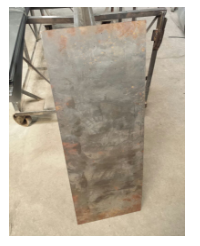
\includegraphics[width=0.4\textwidth]{figures/placa.png}
  \caption{Placa de aço adquirida.}
  \label{fig:placa}
\end{figure}
\FloatBarrier
\par

A serra “tico” e máquina esmerilhadeira foram usadas posteriormente para a realização dos cortes definidos para o contorno da placa e para realizar os dois furos referente as duas entradas de água, conforme a Figura \ref{fig:workers}.

\par
\begin{figure}[h]
  \centering
  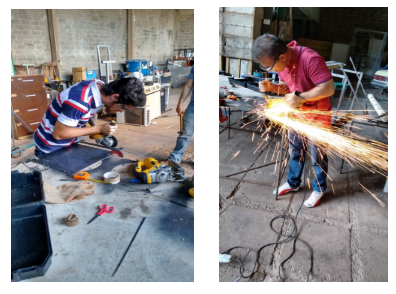
\includegraphics[width=0.7\textwidth]{figures/workers.png}
  \caption{Membros do grupo finalizando a modelagem da placa com a esmerilhadeira.}
  \label{fig:workers}
\end{figure}
\FloatBarrier
\par

Após as modificações a placa adquiriu as mesmas dimensões do sketch pré definido.

\par
\begin{figure}[h]
  \centering
  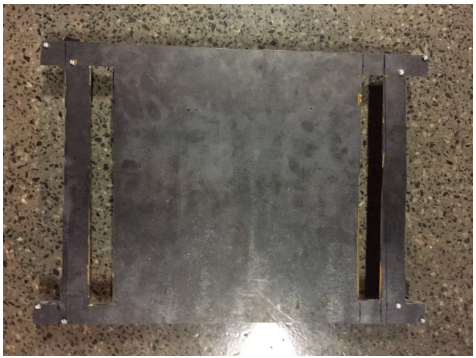
\includegraphics[width=0.6\textwidth]{figures/sketch-base.png}
  \caption{Sketch da base do robô.}
  \label{fig:sketch-base}
\end{figure}
\FloatBarrier
\par

\section{Construção dos Rolos de Limpeza}
Pela dificuldade de se encontrar as escovas, que irão realizar uma das partes da limpeza no processo do \textit{Clean Pool Robot}, a equipe optou por utilizar uma feita pelos integrantes da equipe.

Foi utilizado um tubo cilíndrico de 300x50mm de PVC como base da estrutura dos rolos, e as “cerdas” das escovas foi  utilizado um polímero de fibra de vinil. Esse polimero foi cortado de maneira que seu comprimento fosse o mesmo comprimento da circuferência do tubo de PVC, afim de não existir nenhuma saliência que pudesse prejudicar a limpeza ou movimento do robô.

Para a fixação desse polímero no tubo foi utilizado um adesivo de contato tradicional da marca Cascola para se fazer a união desses dois materiais, depois disso o conjunto polímero e tubo, foi amarrado para que o adesivo estivesse seco e fosse bem aderido para que no momento de uso do robô o polímero não se desprendesse e por consequência não realizasse a escovação. O processo de produção pode ser acompanhado na Figura \ref{fig:rolo}.

\par
\begin{figure}[h]
  \centering
  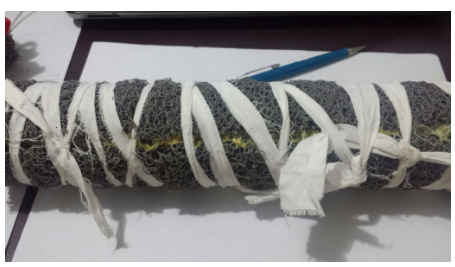
\includegraphics[width=0.5\textwidth]{figures/rolo.png}
  \caption{Processo de fabricação dos rolos de limpeza.}
  \label{fig:rolo}
\end{figure}
\FloatBarrier
\par

Foram confeccionadas duas escovas as quais resultaram na Figura \ref{fig:rolo-fim}.

\par
\begin{figure}[h]
  \centering
  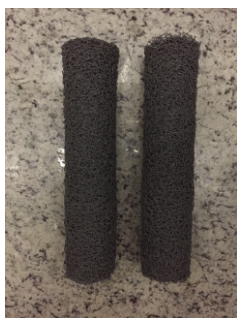
\includegraphics[width=0.35\textwidth]{figures/rolo-fim.png}
  \caption{Rolos de limpeza finalizadas.}
  \label{fig:rolo-fim}
\end{figure}
\FloatBarrier
\par

\section{instalação das Rodas}
Para realizar a instalação das quatro rodas, foi utilizado uma furadeira de bancada onde foram realizados furos para fixação das rodas. Foi utilizado uma broca número 5 e realizado o furo na placa de aço.

\par
\begin{figure}[h]
  \centering
  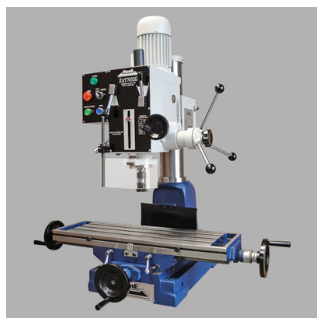
\includegraphics[width=0.5\textwidth]{figures/furadeira.png}
  \caption{Furadeira de bancada utilizada na fixação das rodinhas.}
  \label{fig:furadeira}
\end{figure}
\FloatBarrier
\par

Posteriormente foram fixadas as rodas na placa com parafusos e porcas.

\par
\begin{figure}[h]
  \centering
  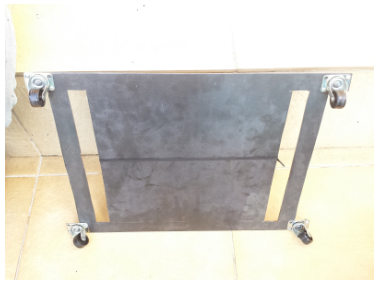
\includegraphics[width=0.7\textwidth]{figures/rodinhas.png}
  \caption{Rodinhas finalizadas na base.}
  \label{fig:rodinhas}
\end{figure}
\FloatBarrier
\par
